\section{Challenges}

Throughout the process, we did face some challenges. We will not present all to you, but some of the most important ones. 

When making the load vector in 3 dimensions, we forgot to map load vector to the right nodes. This resulted in weird displacements, see figure \ref{fig:queens}. and took quite some time to figure out what was wrong. 


\begin{figure}[ht]
        \centering
        \begin{subfigure}[b]{0.45 \textwidth}
                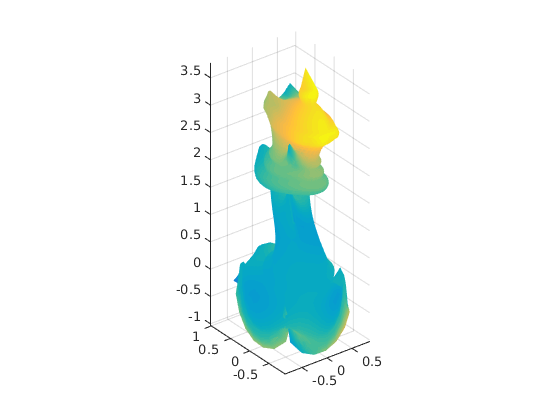
\includegraphics[width=\textwidth]{queen_broken}
                \caption{The chess queen with faulty boundary conditioners.}
        \end{subfigure}
        ~
        \begin{subfigure}[b]{0.45 \textwidth}
                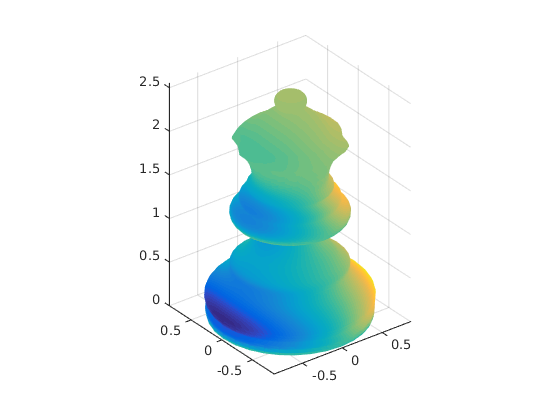
\includegraphics[width=\textwidth]{queen_fixed}
                \caption{The same chess queen with the correct boundary conditions.}
        \end{subfigure}
        \caption{We see that the queen deforms quite badly when dealing with the wrong boundary conditions. }
        \label{fig:queens}
\end{figure}


Also, the matrix \eqref{eq:C} is only valid for an isotropic media, and is thus not valid for wood. Realizing this a little to late, we conclude that the exact same analysis we did could be done with steel, which is isotropic. We also encountered a lot of computational challenges, and some of the improvements can be read about in section \ref{sec:comp}.
